\section*{Method}

In this section, we give an overview of our approach for merging colored de Bruijn graphs that are stored using the $\vari$ data structure, and in the next section, give the merge algorithm in explicit detail.  In both sections, we describe how to merge two colored de Bruijn graphs but note that it generalizes to an  arbitrary number of graphs.  Hence,  we assume that we have two de Bruijn graphs $G_1 = (V_1, E_1)$ and $G_2 = (V_2, E_2)$ as input, which are stored as $\EBWT(G)_1$, $\B_{L1}$, $\B_{F1}$ and $\C_1$ and $\EBWT(G)_2$, $\B_{L2}$, $\B_{F2}$ and  $\C_2 $, respectively.  We will output the merged graph $G_M = (V_M, E_M)$ stored in the same format as the input, more descriptively:  a set of abbreviated edge labels $\EBWT(G)_M$, a bit vector that delimits their common origins $\B_{LM}$, the array $\B_{FM}$, and the color matrix $\C_M$. %storing \(|\{d\,:\,d \in E,\ \elabel (d) \prec c\}|\)
% \(|\{h\,:\,\EBWT(G)[h] \prec c\}|\)
%for each character $c$,  


\subsection*{A Naive Merge Algorithm}

We begin by describing a naive merge procedure to motivate the use of the succinct merge algorithm. We recall from Section \ref{prel:vari} that $\vari$ does not store the edge labels ($k$-mers) of $G$--rather, they have to be computed from the succinct representation.  We denote the edge labels for $G_1$, $G_2$, and $G_M$ as $\L_1$, $\L_2$, and $\L_M$, respectively.  For example, if we want to reconstruct the $k$-mer {\tt AGAGAGTTA} contained in $G_1$ which is stored as {\tt A} in $\EBWT(G)_1$, we need to backward navigate in $G_1$ from the edge labeled {\tt A} through $k-1$ predecessor edges ({\tt T}, {\tt T}, {\tt G},...). We concatenate the abbreviated edge labels encountered during this backward navigation in reverse order to construct the label {\tt AGAGAGTTA}.  Thus, we could naively merge $G_1$ and $G_2$ by reconstructing  $\L_{1}$ and $\L_{2}$, merging them into $\L_{M}$ and computing the succinct representation of $\L_{M}$, i.e., $\EBWT(G)_M$.   We note that this algorithm requires explicitly building $\L_1$, $\L_2$ and $\L_M$ and thus, has a significant memory footprint.  See Algorithm \ref{alg:naive_alg} for pseudocode of this algorithm. 

\begin{figure*}[h!]
\begin{subfigure}[c]{0.5\textwidth}
        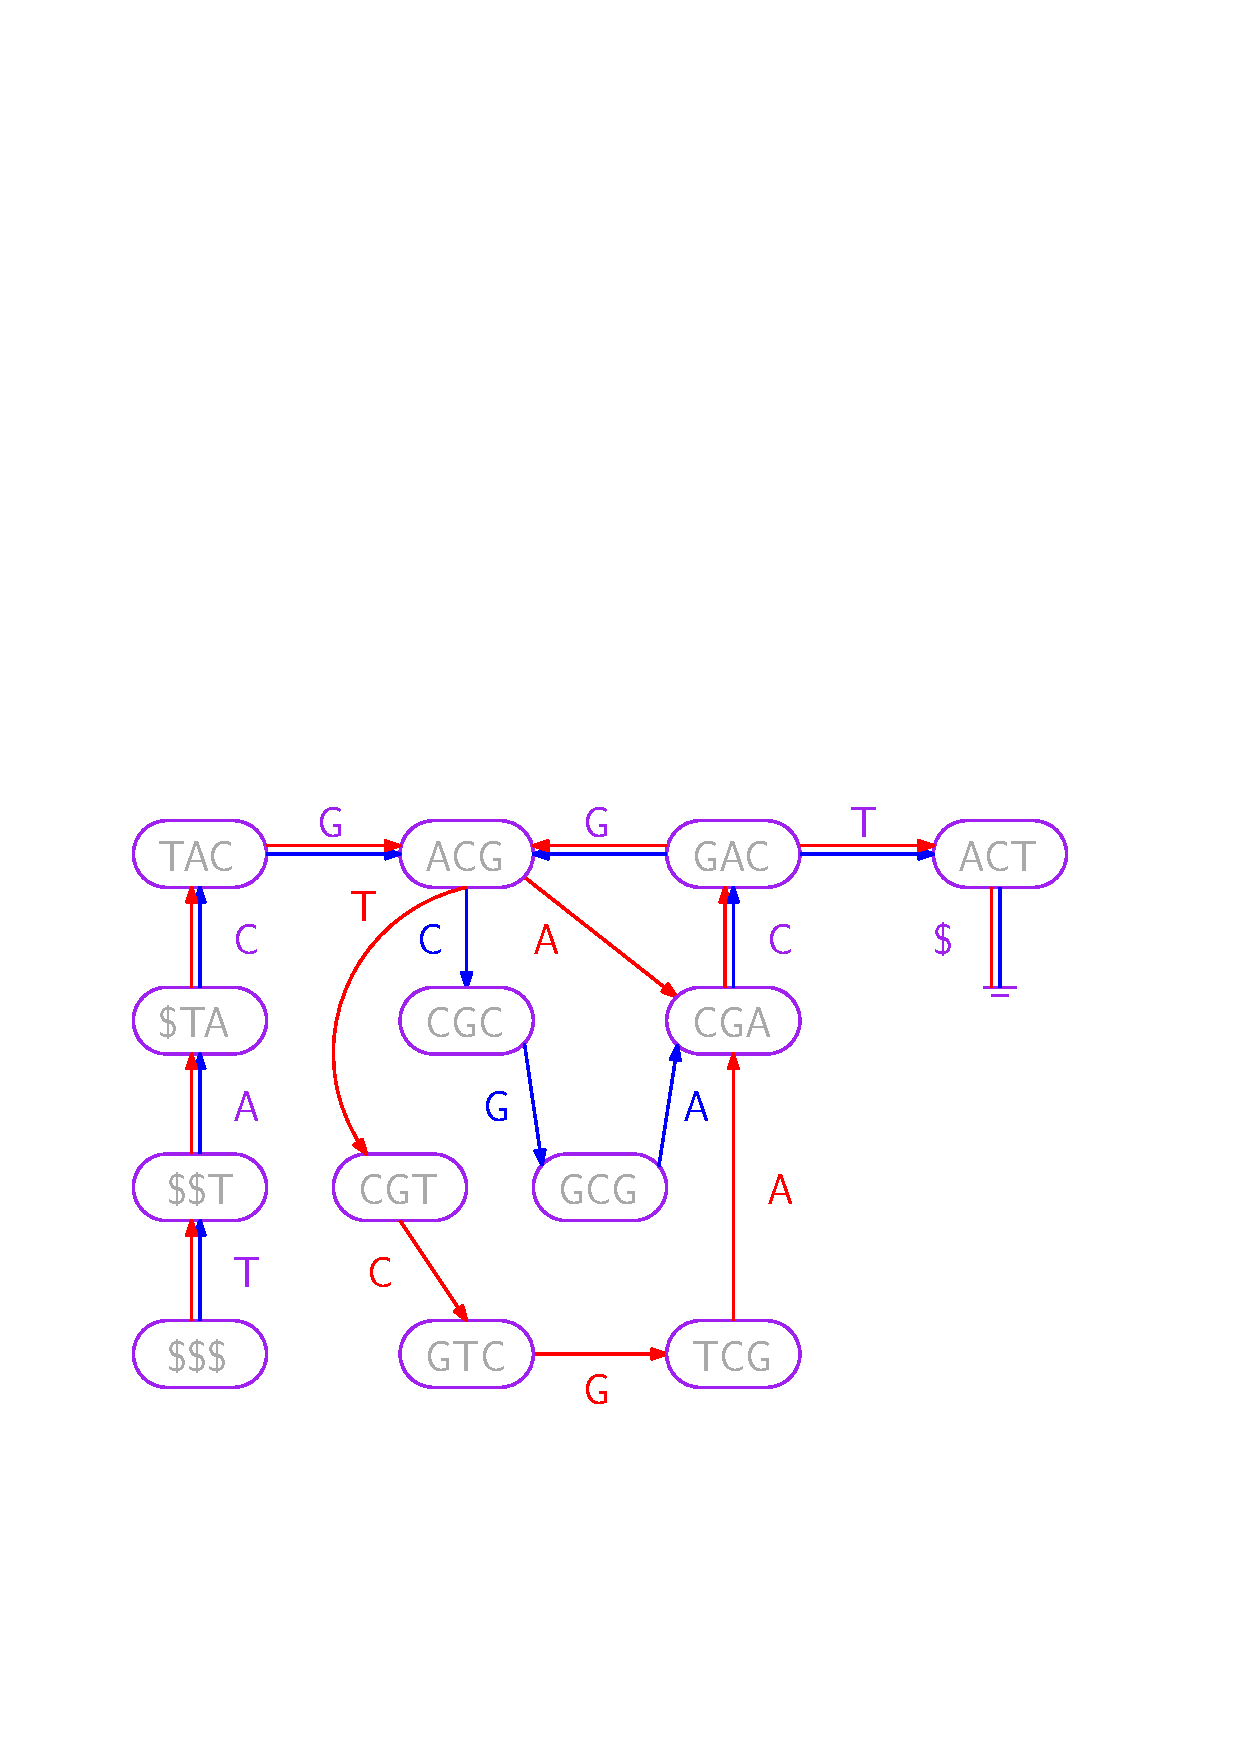
\includegraphics[width=0.9\textwidth]{purplegraph.pdf}
        \caption{A colored de Bruijn graph $G_1$.}
        \label{fig:g1}
    \end{subfigure}
\begin{subfigure}[c]{0.4\textwidth}
        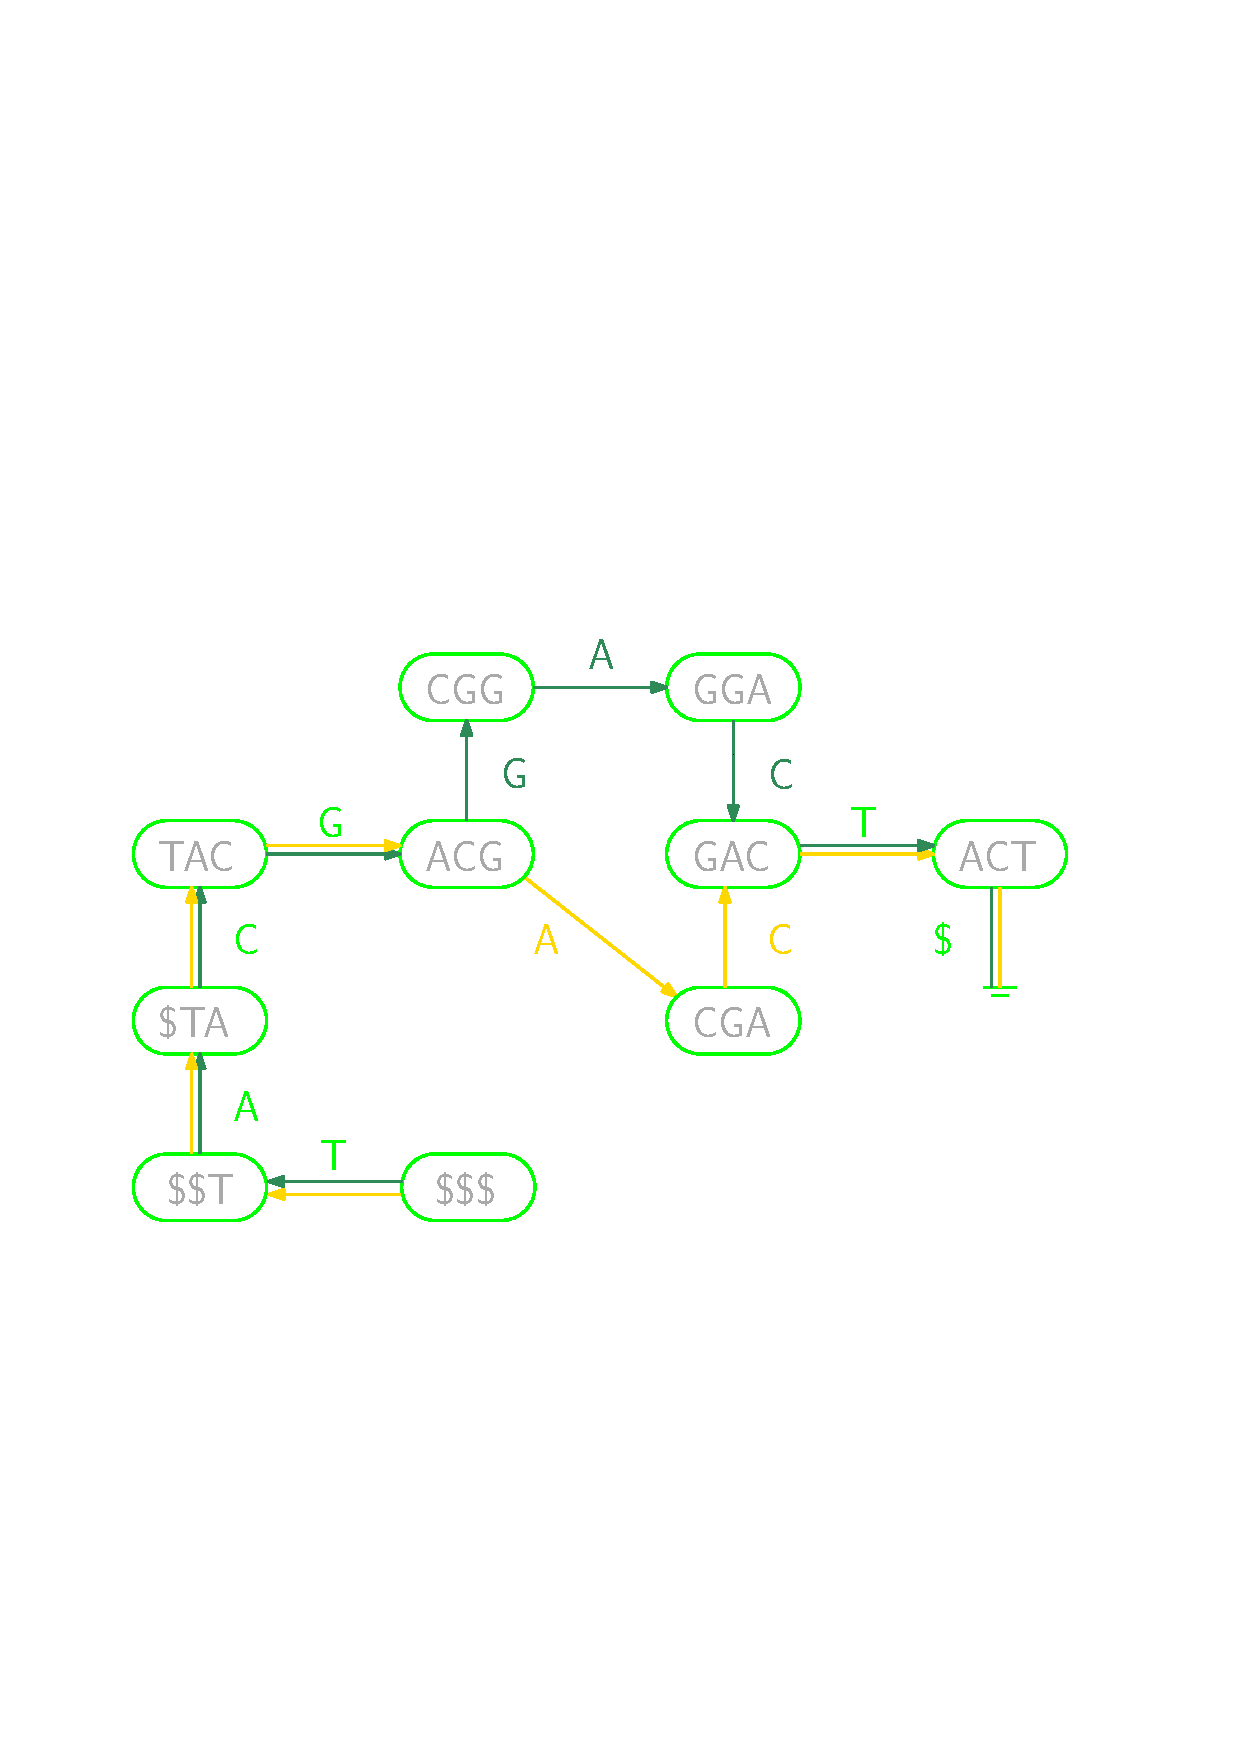
\includegraphics[width=0.9\textwidth]{limegraph.pdf}
        \caption{A second colored de Bruijn graph $G_2$.}
        \label{fig:g2}
    \end{subfigure}
   
\begin{subfigure}[c]{0.5\textwidth}
        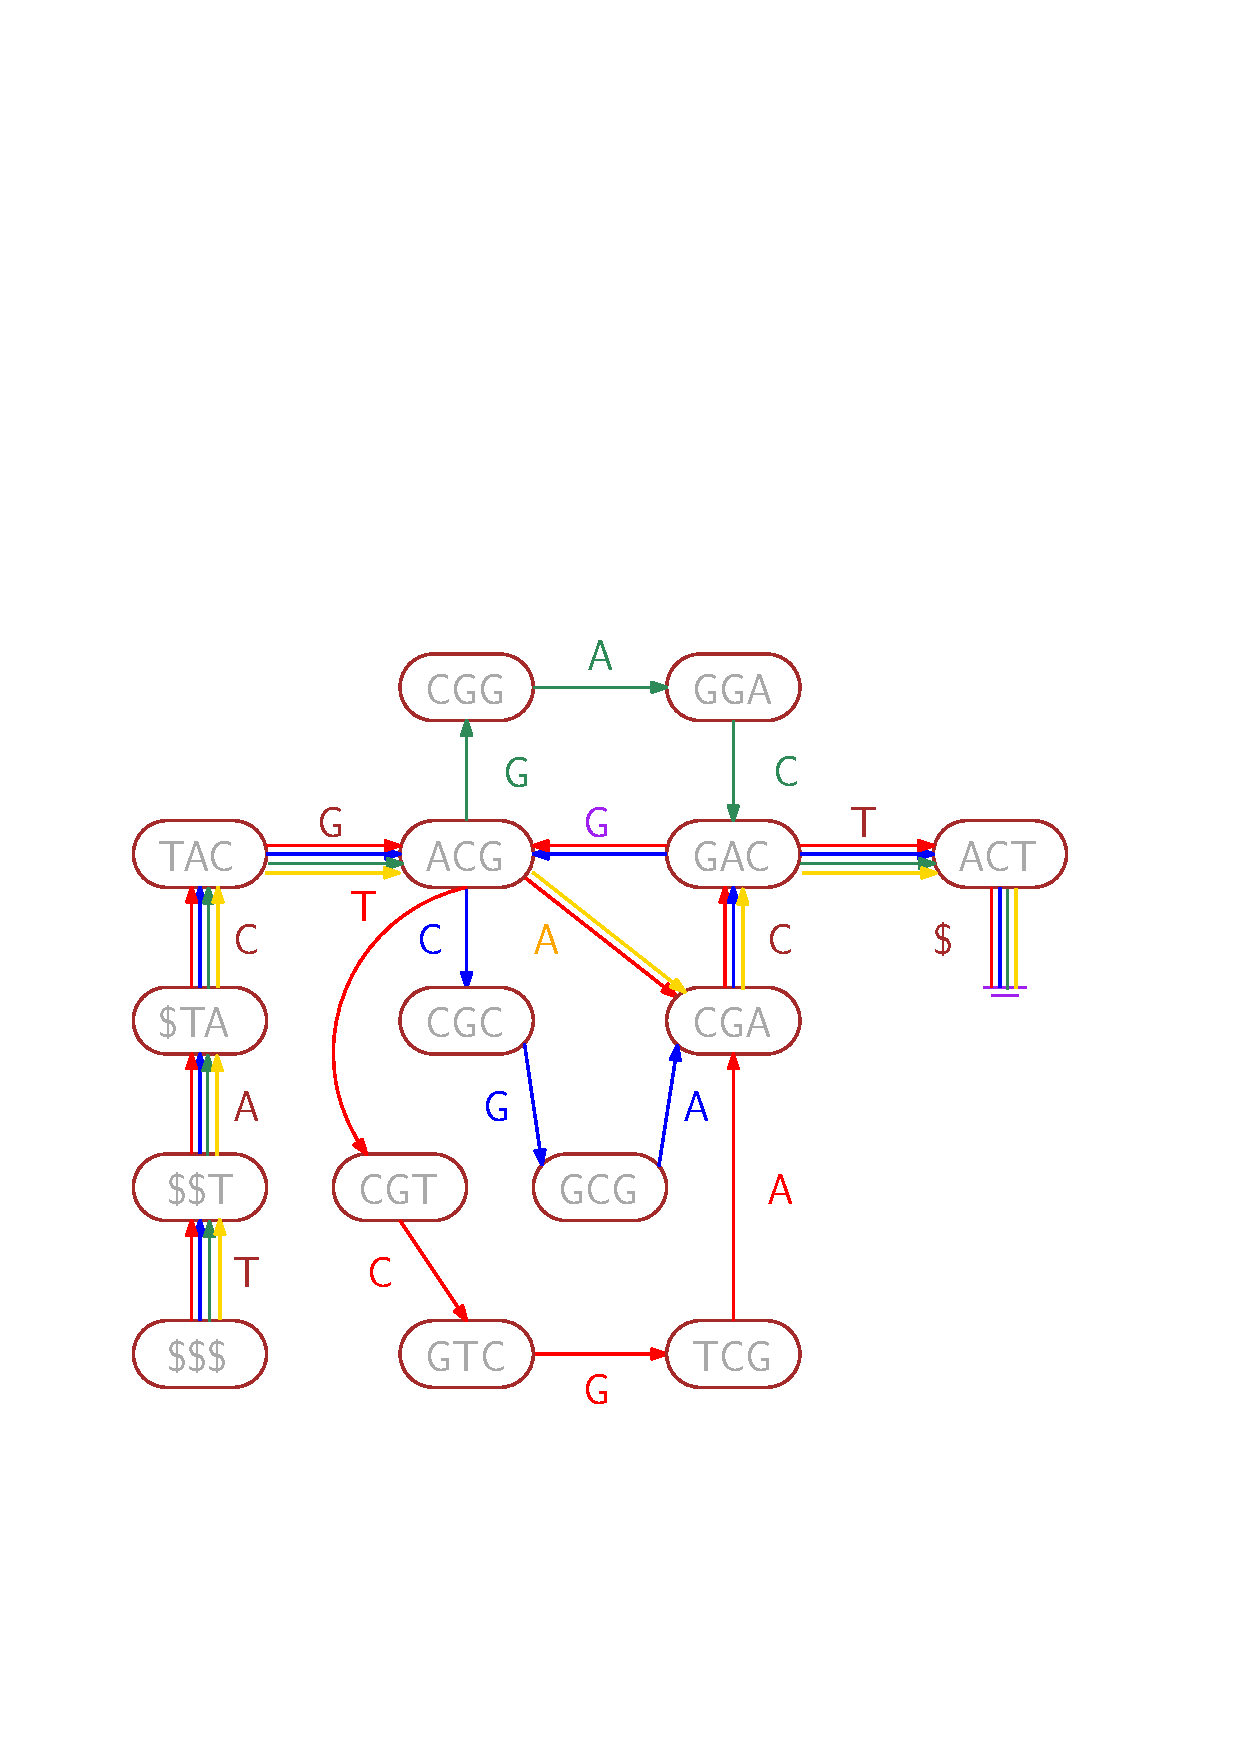
\includegraphics[width=0.95\textwidth]{browngraph.pdf}       
        \caption{The merged colored de Bruijn graph $G_M$.}
        \label{fig:g2}
    \end{subfigure}
\begin{subfigure}[c]{0.5\textwidth}
        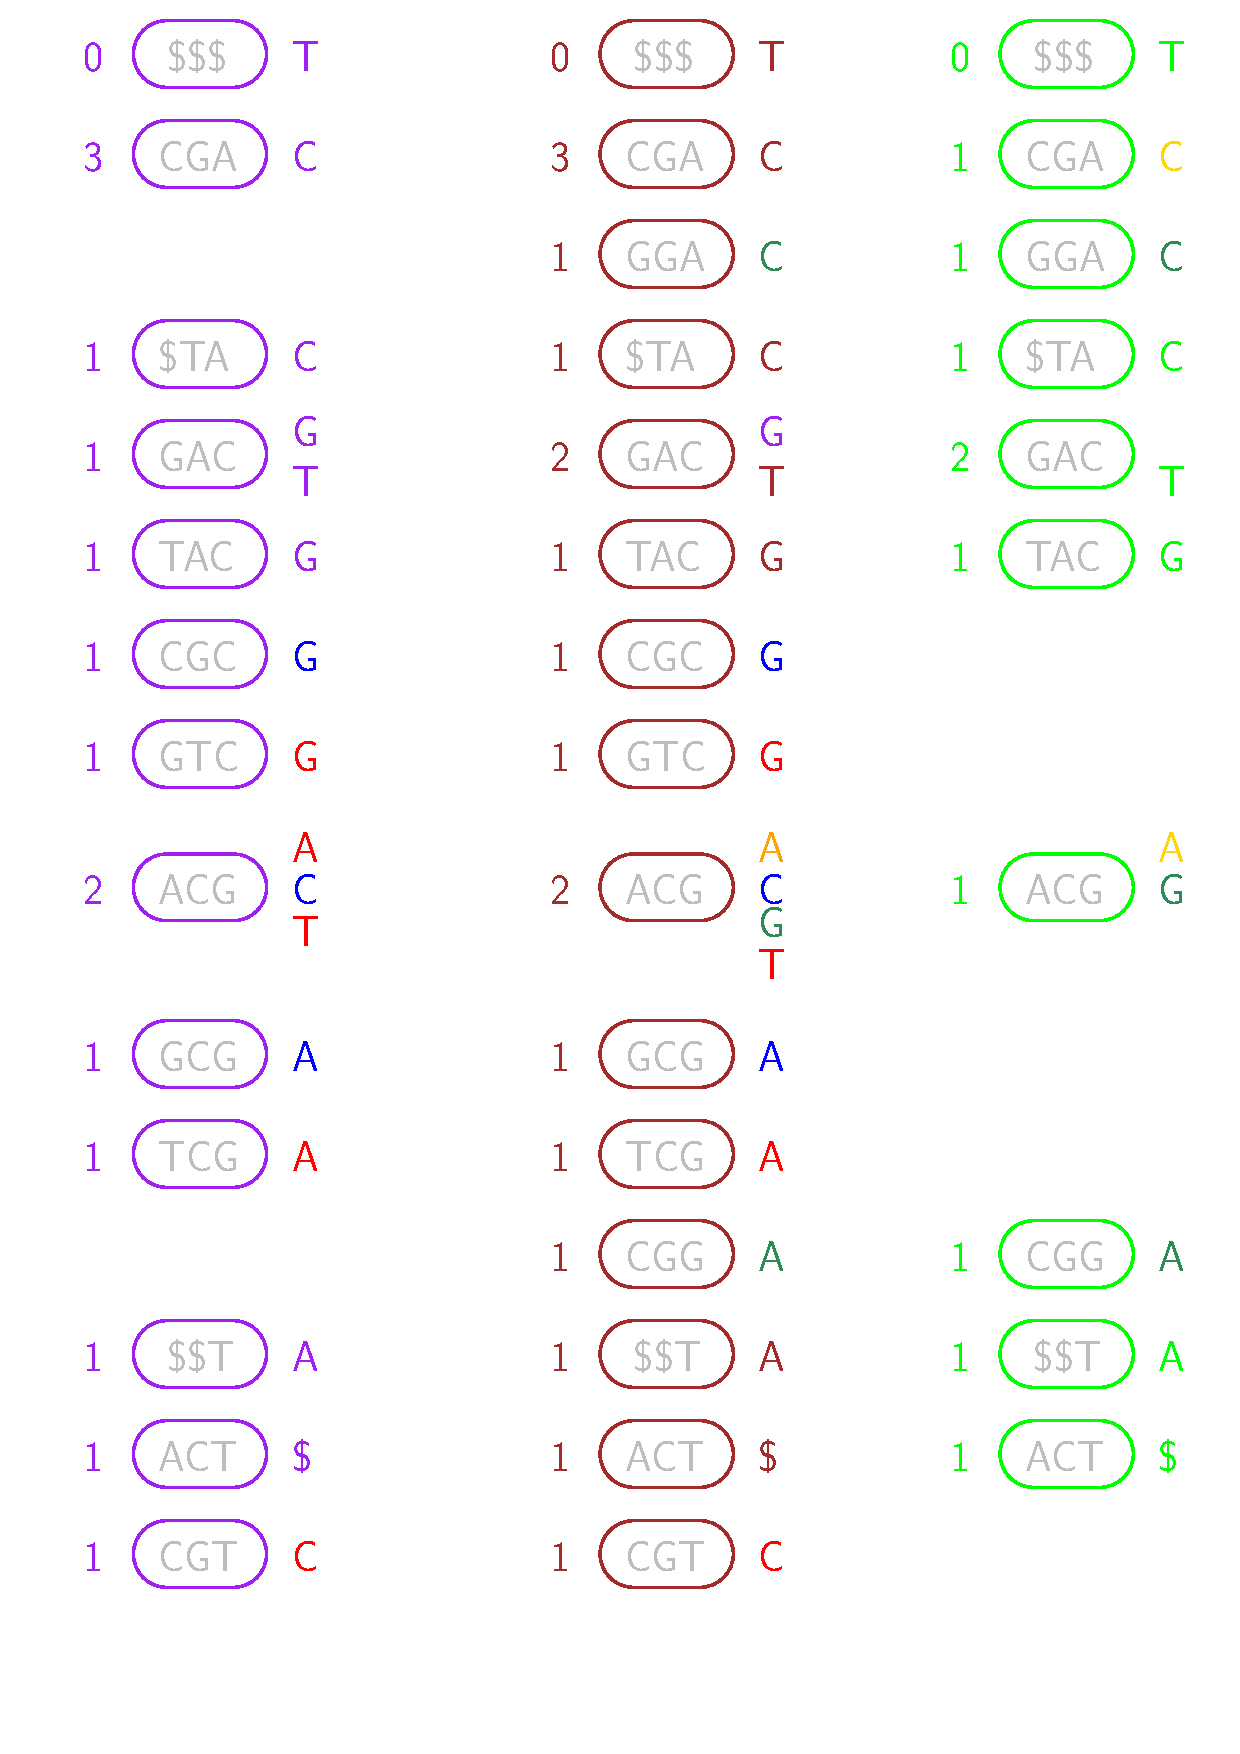
\includegraphics[width=0.9\textwidth]{newbrownmapping.pdf}
        \caption{The representation of the merged colored de Bruijn graph.}
        \label{fig:g2}
    \end{subfigure}
\caption{{\bf (a):} A colored de Bruijn graph consisting of two individual graphs, whose edges are shown in red and blue.  (We can consider all nodes to be present in both graphs, so they are shown in purple.)  {\bf (b):} A second colored de Bruijn graph, whose edges are green and yellow and lime represents presence in both graphs.  {\bf (c) :} A colored de Bruijn graph merged from the two colored de Bruijn  graphs.  {\bf (d):} The nodes for all three graphs arranged in columns (red and blue, merged, green and yellow). Each column is sorted into co-lexicographic order, with each node's number of incoming edges shown on its left and the labels of its outgoing edges shown on its right.  Vertical alignment illustrates how the merged components (center) are copied from either the left, the right, or both.} 
\label{fig:brown}
\end{figure*}


\renewcommand{\algorithmiccomment}[1]{\hskip0em$\triangleright$ #1}

\begin{algorithm}[h!]
\caption{Naive Merge Algorithm.  Because $\L_1$ and $\L_2$ are explicitly constructed a large amount of memory is needed.}
\label{alg:naive_alg}
  \begin{algorithmic}
    \State $\L_1 \leftarrow \emptyset$
    \State $\L_2 \leftarrow \emptyset$
  	\State Populate $\L_1$ and $\L_2$ (See ``Label Recovery'' of Subsection \ref{prel:vari})
	\State Merge $\L_1$ and $\L_2$ into $\L_M$.
	\State Create  $\EBWT(G)_M$, $\B_{LM}$, $\B_{FM}$ from $\L_M$
    \State Create $\C_M$ from $\C_1$ and $\C_2$
	\end{algorithmic}
\end{algorithm}





\subsection*{The Succinct Merge Algorithm}

We are now ready to describe the merge algorithm used as a component of $\ours$.  The trick of the merge algorithm is to build the succinct data structure for $G_M$  without constructing $\L_1$ and $\L_2$, which will in turn reduce memory costs enormously.   


\subsubsection*{Intuitive Explanation of Succinct Merging.} Before we give a detailed explanation of our algorithm we take a step back--abstract away the complexities of the succinct de Bruijn graph--and consider the simpler problem of merging two sorted lists of strings with the constraint that we can only examine a single character from each string at a time.  We can solve this problem with a divide and conquer approach.  First, we group all the strings in each list by their first character.  This partially solves the problem, as we know all the strings in the first group from each list must occur in the output before all the strings in the second group in each list and so on.  Thus, the problem is now reduced to merging the strings in the first group, followed by merging the strings in the second group and so on.  Each of these merges can be addressed by again grouping the elements (i.e. subgroups of the initial groups) by examining the second character of each string.  We can apply this step recursively until all characters of each string have been examined.  

We draw the reader's attention to the fact our succinct colored de Bruijn graph representation is a space-efficient representation of the list of sorted $k$-mers (and $(k - 1)$-mers).  Thus, we can apply this general algorithm but alter it in in the following ways: 1) the nested grouping of the strings is rather a flat partitioning of the two lists into intervals, which is updated each time a character is processed, and 2) the actual merging is reserved for the end once all characters have been processed and their needed information accumulated into set of partitions of each list.

\subsubsection*{Overview of the Algorithm.}

Now we return to the problem of merging succinct colored de Bruijn graphs.  We refer to $\EBWT(G)_M$ and $\C_M$ as the {\em primary components} of the data structure and $\B_{FM}$ and $B_{LM}$ as {\em secondary components}.  We describe how to merge the primary components, and leave the details of how to merge the secondary components to the supplement.   The algorithm consists of two steps: (1) a planning step which plans the merge, and (2) a final execution step which executes the planned merge. In the planning step, we output a list of non-overlapping intervals for $\L_{1}$ and one for $\L_{2}$.  We refer to these lists as a {\em merge plan}, which is then used to execute the merge.  There are $k$ iterations of the planning algorithm (where $k$ corresponds to the $k$-mer value).  At each iteration of the algorithm a single character of the edge labels ($k$-mers) is processed, and the merge plan is revised. After $k$ iterations, we execute the merge plan.


\subsubsection*{The Planning Step.}  

We denote the merge plan as $P_1 = \{[0, p^1_1],...,[p^1_i, |\L_{1}|]\}$ where each $p^1_1,..,p^1_i$ is an index in $\L_{1}$, and $P_2 = \{[0, p^2_1],...,[p^2_i, |\L_{2}|]\}$, where each $p^2_1,..,p^2_i$ is an index in $\L_{2}$.   We first initialize $P_1$ and $P_2$ to be single intervals covering $\L_1$ and $\L_2$, respectively (e.g. $P_1 = \{[0, |\L_1|]\}$ and  $P_2 = \{[0, |\L_2|]\}$). Next, we revise $P_1$ and $P_2$ in an iterative manner.  In particular, we perform $k$ consecutive revisions of $P_1$ and $P_2$, where $k$ is the $k$-mer value used to construct $G_1$ and $G_2$---each revision of $P_1$ and $P_2$ is based on the next character\footnote{We recall that FM-index stores the last character of each edge label and we do not have access to $\L_1$ and $\L_2$.  Therefore, we are processing the characters of $\L_1$ and $\L_2$ from right to left.  Thus, the ``next'' character is the preceding character of an edge label.} of each edge label in $\L_1$ and $\L_2$.  An overview of the The Planning Step is given in Algorithm \ref{alg:mergeplan}.  Thus, in order to fully describe the planning stage, we define (1) how the characters of the edge labels are computed (e.g. $\emph{GetCol}(i, G_1)$ in Algorithm \ref{alg:mergeplan}), and (2) how $P_1$ and $P_2$ are revised based on these characters (e.g. $\emph{RefinePlan}(P_1, P_2, Col_1, Col_2, i)$ in Algorithm \ref{alg:mergeplan}). 


\begin{algorithm}[h!]
\caption{The planning step to merge $G_1$ and $G_2$. } %We use the convention in this presentation that list values are indexed from $[1..|list|]$, as opposed to starting at 0. }
\label{alg:mergeplan}
\begin{algorithmic}
%  \Procedure{PlanningStep}{$G_1$, $G_2$}
    
  \State \Comment{Initialize plan to single intervals covering entire $EBWT(G)$s.}
  \State $P_1 \leftarrow ([1, |EBWT(G)_1|])$
  \State $P_2 \leftarrow ([1, |EBWT(G)_2|])$

 % \State \Comment{Iterate through ``edge label matrix'' columns in sort precedence order}
  \ForAll{$i \in \{1..k\}$}
    \State $Col_1 \leftarrow \emph{GetCol}(i, G_1)$
    \State $Col_2 \leftarrow \emph{GetCol}(i, G_2)$

  \State \Comment{``RefinePlan'' is given in the supplement.}
    \State $(P_1', P_2') \leftarrow \emph{RefinePlan}(P_1, P_2, Col_1, Col_2, i)$
    \State $(P_1, P_2) \leftarrow (P_1', P_2')$
    \EndFor
 %   \EndProcedure
\end{algorithmic}

\end{algorithm}


\paragraph{Computing the next character of $\L_1$ and $\L_2$.}   

We let $i$ denote the current iteration of our revision of $P_1$ and $P_2$, where $1 \leq i < k$. We compute the next characters of $\L_1$ and $\L_2$ using two temporary character vectors $Col_1^i$ and $Col_2^i$, which are of length $|\L_1|$ and $|\L_2|$, respectively.    Conceptually, we define these vectors as follows: $Col_1^i[j] = \L_1[j][k-i]$ if $j < k$ and otherwise $Col_1^i[j] = \L_1[j][k]$, and $Col_2^i[j] = \L_2[j][k-i]$ if $j < k$; and otherwise $Col_2^i[j] =  \L_2[j][k]$. Since we do not explicitly build or store $\L_1$ and $\L_2$, we must compute $Col_1^i$ and $Col_2^i$.  We leave the details of computing $Col_1^i$ and $Col_2^i$ based on the succinct de Bruijn graph to the supplement (see Subsection 1).

% This computation follows the Label Recovery algorithm that was described in  Subsection \ref{prel:vari}. 
 


\paragraph{Revising $P_1$ and $P_2$.}
We revise $P_1$ and $P_2$ based on $Col_1^i$ and $Col_2^i$ at iteration $i$ by considering each pair of intervals in $P_1$ and $P_2$, i.e., $P_1[n]$ and $P_2[n]$ for $n = 1,.., |P_1|$, and partitioning each interval into at most five sub-intervals.  We store the list of sub-intervals of $P_1$ and $P_2$ as $SubP_1$ and $SubP_2$. Intuitively, we create $SubP_1$ and $SubP_2$ in order to divide $P_1[n]$ and $P_2[n]$ based on the runs of covered characters in  $Col_1^i$ and  $Col_2^i$---e.g., for each run of {\tt A}, {\tt C}, {\tt G}, {\tt T} or {\tt \$} (See Figure 1 in the supplement). Next, we formally define this computation.

Thus, we partition $P_1$ by first computing the subvector of $Col_1^i$ that is covered by $P_1[n]$, which we denote as $Col_1^i(P_1[n])$, and computing the subvector of $Col_2^i$ that is covered by $P_2[n]$, which we denote  as $Col_2^i(P_2[n])$.  Next, given a character $c$ in $\{ {\tt \$},  {\tt A}, {\tt C}, {\tt G}, {\tt T} \}$, we populate $SubP_1[c]$ and $SubP_2[c]$ based on $Col_1^i(P_1[n])$ {\em and} $Col_2^i(P_2[n])$ as follows: (1) we check whether $c$ exists in either $Col_1^i(P_1[n])$ or $Col_2^i(P_1[n])$; (2) if so, we add an interval to $SubP_1[c]$ covering the contiguous range of $c$ in  $Col_1^i(P_1[n])$ (or add an empty interval if $Col_1^i(P_1[n])$ lacks any instances of $c$), and add an interval to $SubP_2[c]$ covering the contiguous range of $c$ in  $Col_2^i(P_1[n])$ (or, likewise, add an empty interval if $Col_2^i(P_1[n])$ lacks any instances of $c$)\footnote{We are guaranteed by the definition of our data structure that any instances of $c$ in $Col_1^i(P_1[n])$ will be in a contiguous range, and likewise, any instances of $c$ in $Col_2^i(P_1[n])$ will also be in a contiguous range}.  Finally, we concatenate all the lists in $SubP_1$ and $SubP_2$ to form the revised plan $P_1'$ and $P_2'$. This revised plan $P_1'$ and $P_2'$ becomes the input $P_1$ and $P_2$ for the next refinement step. We refer the reader to Algorithm 2 in the supplement for the pseudocode. 
  
We crafted the method above to maintain the property described in the following observation.  %The first condition states that the size of the two lists of intervals remains the same.  The second condition implies that if two elements are in separate intervals in $P_1$ or $P_2$ then they remain in separate intervals after they are revised. Lastly, the third condition implies that the revision of $P_1$ and $P_2$ will divide any interval into at most five subintervals.  Hence, this observation implies that at each iteration of the algorithm will further partition the elements of $\L_1$ and $\L_2$ relative to the previously processed ($q+1$) position.

 
\begin{observation} \label{obs} Let $P_1$ be a (partial) merge plan, and $P_1'$ its refinement by our merge algorithm, where $\ell_1,..,\ell_n$ are the elements in $\L_1$ that are covered by interval $p_{i} \in P_1$ and $m_1,...,m_o$ are the  elements of $\L_2$ covered by interval $q_{j} \in P_2$.  The following conditions hold:  (1) $|P_1| = |P_2|$ and $|P_1'| = |P_2'|$; (2) given any pair of
% In english, I would say "is covered by" where we use $\in$.  
  elements where $\ell_a \in p_i$, $\ell_b \in p_j$ and $p_i \cap p_j = \emptyset$ there exists intervals $p_i'$ and $p_j'$ in $P_1'$ such that  $p_i' \cap p_j' = \emptyset$ and  $\ell_a \in p_i'$, $\ell_b \in p_j'$; and lastly, (3) given an interval $p_i$ in $P_1$ and the subsets of the alphabet used $\sigma_1 \in \ell_1,..,\ell_n$ and $\sigma_2 \in m_1,...,m_o$, then $p_i$ will be partitioned into $|SubP_1| = |\sigma_1\cup\sigma_2|$ subintervals in $P_1'$.
\end{observation} 

We defined this observation for $P_1$ but note that an analogous observation exists for $P_2$.


%\begin{algorithm}[h!]
%\caption{Revising $P_1$ and $P_2$} %We use the convention in this presentation that list values are indexed from $[1..|list|]$, as opposed to starting at 0. }
%\label{alg:mergeplan}

  %\begin{algorithmic}
      
    %\State $P_1' \leftarrow ()$
    %\State $P_2' \leftarrow ()$
    %\State \Comment{For each interval in $P_1$ (and $P_2$)}
    %\ForAll{$j \in \{1..|P_1|\}$}
    %  \State \Comment{...extract a window from each column covered by the interval...}
    %  \State $W_1 \leftarrow \emph{CoveredSymbols}(Col_1, P_1[j])$
     % \State $W_2 \leftarrow \emph{CoveredSymbols}(Col_2, P_2[j])$
     % \State \Comment{...and partitioning that window on its character runs, forming sub-intervals.}
     % \State $(SubP_1, SubP_2) \leftarrow \emph{Partition}(W_1, W_2)$
     % \State $P_1'.\emph{Concatenate}(SubP_1)$
     % \State $P_2'.\emph{Concatenate}(SubP_2)$
     % \EndFor
     % \State \Comment{Capture snapshots of important intermediate plan states.}
     % \If {$i \in \{1, k-1, k-2\}$ }
     %   \State $S_{i} \leftarrow (P_1', P_2')$
     % \EndIf
     % \State \Return $(P_1', P_2')$
   
%\end{algorithmic}

%\end{algorithm}


\subsubsection*{The Execution Step.} 

We execute the merge plan by combining the elements of $\EBWT(G)_1$ that are covered by an interval in $P_1$ with the elements of $\EBWT(G)_2$ that are covered by the equal position interval in $P_2$ into a single element in $\EBWT(G)_M$.  We note that when all characters of each label in $\L_{1}$ and $\L_{2}$ have been computed and accounted for, each interval in $P_1$ and $P_2$ will cover either 0 or 1 element of $\L_{1}$ and $\L_{2}$ and the number of intervals in $P_1$ (equivalently $P_2$) will be equal to $|\EBWT(G)_M|$. Thus, we consider and merge each pair of intervals of $P_1$ and $P_2$ in an iterative manner.  We let  $(p_i^1, p_i^2)$ as the $i$-th pair of intervals.  We concatenate the next character of $\EBWT(G)_1$ onto the end of $\EBWT(G)_M$ if $|p_i^1| = 1$.  If $|p_i^2| = 1$ then we dismiss the next character of  $\EBWT(G)_2$ since it is an abbreviated form of an identical edge to that just added. Next, if $|p_i^1| = 0$ and $|p_i^2| = 1$, we copy the next character from $\EBWT(G)_2$ onto the end of $\EBWT(G)_M$.  We refer the reader to Algorithm 2 for the pseudocode in the supplement.

We merge the color matrices in an identical manner by copying elements of $\C_1$ and $\C_2$ to $\C_M$.  Again, we iterate through the plan by considering each pair of intervals. If $|p_i^1| = 1$ and $|p_i^2| = 1$ then we concatenate the corresponding rows of $\C_1$ and $\C_2$ to form a new row that is added to $\C_M$.  If only one of $p_i^1$ or $p_i^2 $ is non-zero then the corresponding row of $\C_1$ or $\C_2$ is copied to $\C_M$ with the other elements of the new row set to $0$.


\subsection*{Computational Complexity}

The following theorem demonstrates the efficiency of our approach. 

\begin{theorem} Given two de Bruijn graphs $G_1 = (V_1, E_2)$ and $G_2 = (V_2, E_2)$ constructed with integral value $k$ such that, without loss of generality, $|E_1| \geq |E_2|$, it follows that our merge algorithm constructs the merged de Bruijn graph $G_M$ in $O(m \cdot \max(k, t))$-time, where $t$ is the number of colors (columns) in $\C_M$ and $m = |E_1|$. \end{theorem}

\begin{proof}   %We first consider the time required to merge the primary components of the data structure.
  In our merge algorithm, we will perform $k$ refinements of $P_1$ and $P_2$ after they are initialized. We know by definition and Observation \ref{obs} that $|P_1| \leq |\L_1|$,  $P_2 \leq |\L_2|$, $Col_1^i \leq |\L_1|$ and $Col_2^i \leq |\L_2|$ at each iteration $i$ of the algorithm.  Further, it follows from Observation \ref{obs} that a constant number of operations are performed to $P_1$,  $P_2$, $Col_1^i$ and $Col_2^i$. We populate $\C_M$ in the last step of merging the primary components of the data structure.  Since the  $\C_M$ is a bit matrix of size $k$ by $t$, it follows that this step will take time $O(m \max(k, t))$-time.  Hence, if $k \leq t$ the merge algorithm will take $O(mk)$-time; otherwise it will take $O(mt)$-time (since populating $\C_M$ will dominate in this case). 
%  {\color{red} Next, we consider the time required to merge the secondary components. }
\end{proof} 

%\subsection{Implementation Details}

%We store $P_1$ and $P_2$ as unary encoding runs of $0$ bits representing interval lengths, each delimited by a `1' bit. This storage format allows us to perform the merge in a streaming fashion where a `0' bit is read at the same time as one nucleotide from each column, and intervals can be subdivided just by inserting an additional `1' bit in the output.


%\end{methods}
